% TO DO:
% * look up Heike's kronecker product notation
% * complete display considerations
% * complete conclusions and plans for future work

% zip -r graphical-inference.zip *.pdf *.tex images references.bib *.cls

% 8 pages, including reference 
% 
% Frame as design paper:
% 
%   * explain the target problem
%   * enough background that the reader can pass judgement about whether your
%     solution is good
%   * you should present results that back up the claim that your approach is
%     better than others
%
% Supplemental material to create plots
\documentclass[journal]{vgtc}
\usepackage{mathptmx}
\usepackage{graphicx}
\graphicspath{{plots/}}
\usepackage{times}
\usepackage{booktabs}
\usepackage[utf8]{inputenc}
\usepackage[square,sort&compress]{natbib}

\usepackage{tikz}
\definecolor{female}{HTML}{EF8A62}
\definecolor{male}{HTML}{67A9CF}
\definecolor{not-too-happy}{HTML}{FC8D59}
\definecolor{pretty-happy}{HTML}{FFFFBF}
\definecolor{very-happy}{HTML}{91CF60}
\definecolor{not-too-happy}{HTML}{FC8D59}
\definecolor{pretty-happy}{HTML}{FFFFBF}
\definecolor{very-happy}{HTML}{91CF60}
\definecolor{married}{HTML}{F1EEF6} 
\definecolor{never-married}{HTML}{BDC9E1} 
\definecolor{divorced}{HTML}{74A9CF} 
\definecolor{widowed}{HTML}{2B8CBE} 
\definecolor{separated}{HTML}{045A8D} 
\definecolor{grey30}{HTML}{4D4D4D}
\newcommand{\key}[1]
  {\protect \tikz{\fill[#1] rectangle (1ex,1ex);}}

\newcommand{\includegraphicsinline}[2]{\begin{minipage}{#1}\includegraphics[width=\linewidth]{#2}\end{minipage}}

\onlineid{0}
\vgtccategory{Research}
\vgtcinsertpkg

\title{Product plots}
\author{Hadley Wickham, and Heike Hofmann}
\authorfooter{
  \item Hadley Wickham is an Assistant Professor of Statistics at Rice University, Email: hadley@rice.edu.
  \item Heike Hofmann is an Associate Professor of Statistics at Iowa State University.
}
\shortauthortitle{Wickham \MakeLowercase{\textit{et al.}}: Product plots}

\abstract{We propose a new framework for visualising tables of counts, proportions and probabilities. We call our framework product plots, alluding to the computation of area as a product of height and width, and the statistical concept of generating a joint distribution from the product of conditional and marginal distributions. The framework, with extensions, is sufficient to encompass over 20 visualisations previously described in fields of statistical graphics and infovis, including bar charts, mosaic plots, treemaps, equal area plots and fluctuation diagrams.}

\keywords{Statistics, joint distribution, conditional distribution, treemap, bar chart, mosaic plot}
\CCScatlist{ % not used in journal version
  \category{H.5.2}{Information Interfaces and Presentation}{ User Interfaces --- Graphical user interfaces (GUI), Interaction styles, Screen design, Evaluation/methodology}
  \CCScat{I.6.8}{Computing Methodologies}%
  {Simulation and Modeling}{Visual Simulation};
}

\teaser{
\centering
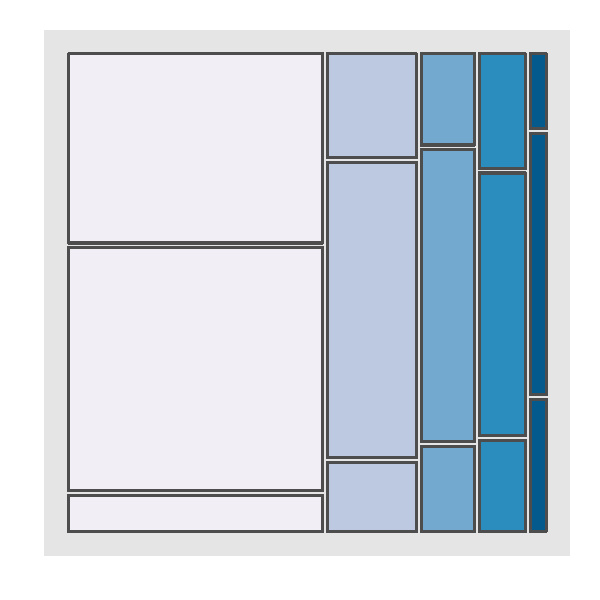
\includegraphics[width=0.16\linewidth]{banner-1}%
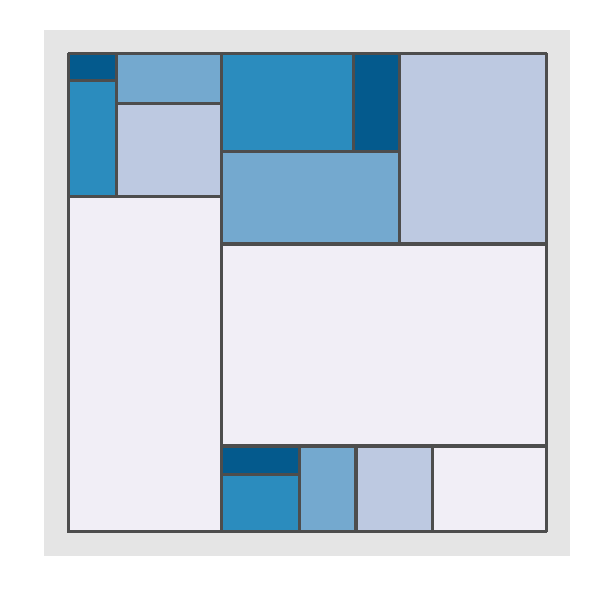
\includegraphics[width=0.16\linewidth]{banner-2}%
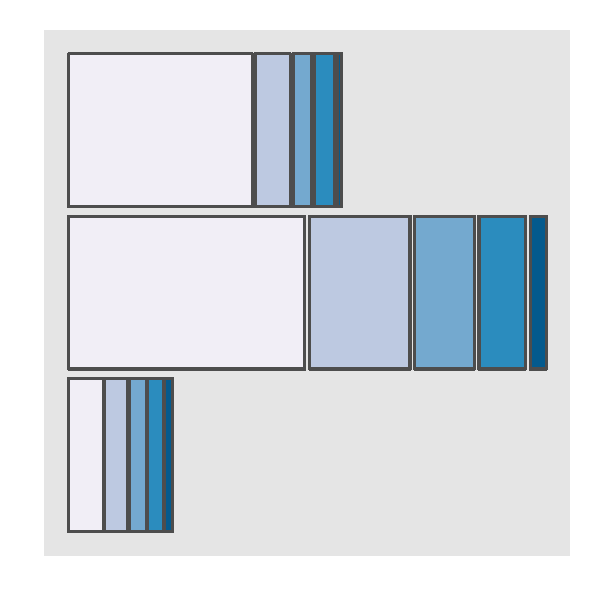
\includegraphics[width=0.16\linewidth]{banner-5}%
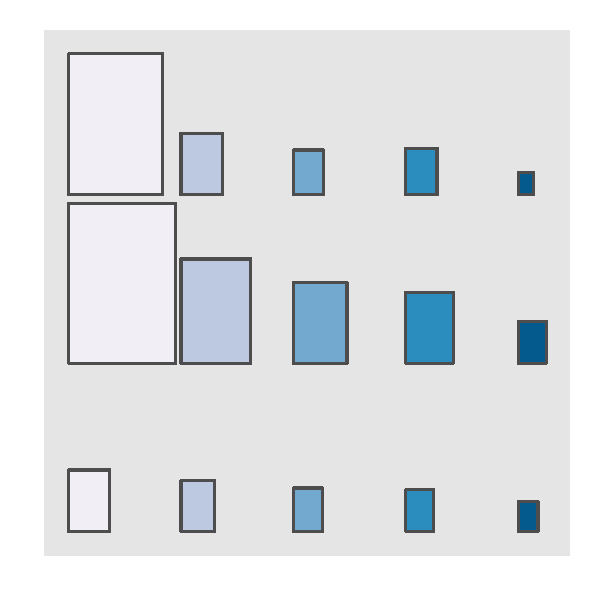
\includegraphics[width=0.16\linewidth]{banner-6}%
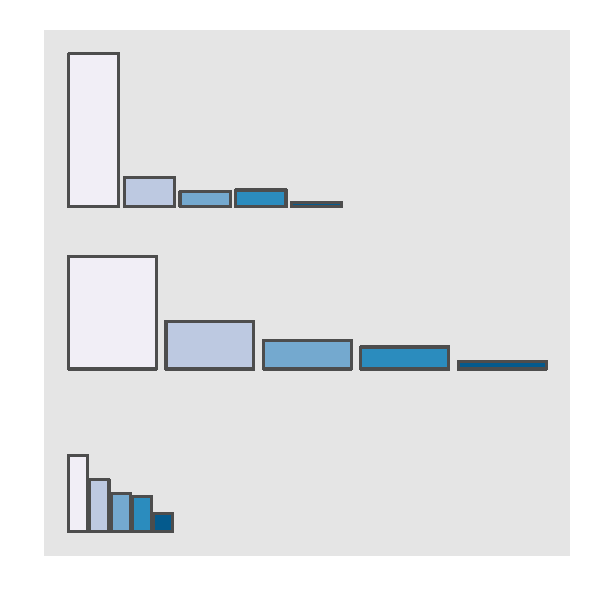
\includegraphics[width=0.16\linewidth]{banner-3}%
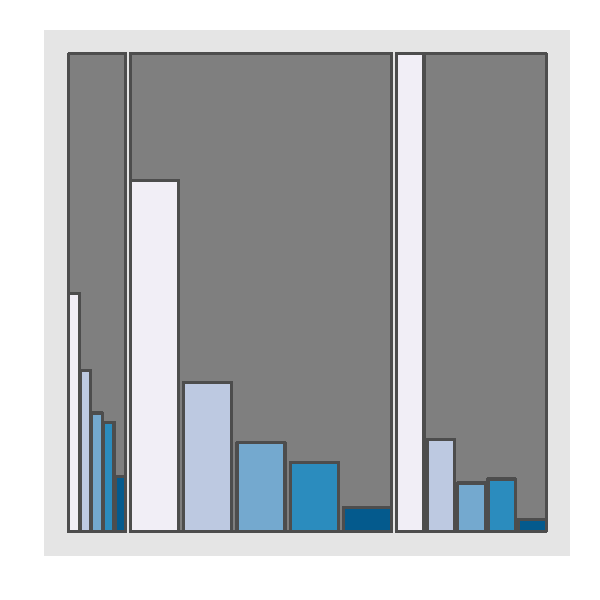
\includegraphics[width=0.16\linewidth]{banner-4}
\caption{A selection of plots encompassed by the product plots framework.  All display the same data (the distribution of happiness and marital status), but each supports a different question. From left to right: mosaic plot, treemap, stacked  bar chart, fluctuation diagram, and two new plots that don't have names. In all plots, area is proportional to probability. }
\label{fig:teaser}
}

\renewcommand{\manuscriptnotetxt}{\itshape Manuscript received 31 March 2011; accepted XX XXXX XXXX; posted online XX XXXX XXXX; mailed on XX XXXX XXXX. 

For information on obtaining reprints of this article, please send email to: tvcg@computer.org.}


\begin{document}
\firstsection{Introduction}
\maketitle

Tables of counts, proportions and probabilities are an extremely common form of data, and many researchers have developed visualisations to display them. In this paper, we develop a framework that encompasses many existing visualisations, from bar charts to treemaps to pie charts, showing how graphics that previously seemed unrelated in fact share a deep underlying connection \citep{cox:1978}. Our framework makes it easier to describe and create visualisations of categorical data, shows how existing methods are related and where new methods can be developed, and will make it easier to match questions about categorical data to the visualisations that will provide revealing answers.

Our framework focusses on area charts, where the area of a graphical element is proportional to the underlying count, proportion, or probability. We call our framework \emph{product plots} in allusion to two products: the product of width and height to generate area, and the product of conditional and marginal distributions to produce joint distributions. A key development of the products plot framework is the inverse operation: the factorisation of high-dimensional data to products of low-dimensional plots. This allows us to  combine simple, low-dimensional graphical primitives to display complex, high-dimensional data.

We begin in Section~\ref{sec:primitives} by motivating the three constraints that give rise to the basic graphical component of product plots: the rectangle. We constrain the rectangle further to produce three 1d atoms (bar, spine, tile) and one 2d atom (the fluct). These constraints will later be relaxed in Section~\ref{sec:variations} to extend our framework to include more visualisations such as histograms, pie charts, cascaded treemaps and weighted plots.

Section~\ref{sec:combination} provides the mathematical framework that allows us to combine the 1d and 2d atoms to display data of any dimensionality. This framework is based on the fundamental statistical idea that any high dimensional distribution can be factorised into a product of low-dimensional conditional and marginal distributions. Section~\ref{sec:existing} shows how many existing named graphics are special cases of this general pattern.

Section~\ref{sec:display} discusses some considerations for the display of product plots, and Section~\ref{sec:package} introduces the R package {\tt prodplot}, our reference implementation of the product plots framework. Finally, Section~\ref{sec:conclusion} discusses our plans for the future.

To illustrate these ideas, we will use the same data in all examples. The data is a small sample of variables related to happiness from the general social survey ({\sc gss}) \citep{davis:2008}. The {\sc gss} is a yearly cross-sectional survey of Americans, run from 1976. We combine data for 25 years to yield 51,020 observations, and of the over 5,000 variables, we select nine related to happiness, as described in Table~\ref{tbl:happy}.

\begin{table*}[htb]
  \centering
  \begin{tabular}{llp{9cm}}
    \toprule
    Variable & Description & Values \\
    \midrule
    {\sf age} & age in years & 18--89 \\
    {\sf degree} & highest education & lt high school, high school, junior college, bachelor, graduate \\
    {\sf finrela} & relative financial status & far above, above average, average, below average, far below \\
    {\sf happy} & happiness & \key{very-happy} very happy, \key{pretty-happy} pretty happy, \key{not-too-happy} not too happy \\
    {\sf health} & health & excellent, good, fair, poor \\
    {\sf marital} & marital status & \key{married} married, \key{never-married} never married, \key{divorced} divorced, \key{widowed} widowed, \key{separated} separated \\
    {\sf sex} & sex & \key{female} female, \key{male} male\\
    {\sf wtsall} & probability weight & 0.43--6.42 \\
    {\sf year} & year of survey & 1972--2006 \\
    \bottomrule
  \end{tabular}
  \caption{Description of sample data. Common plot colours are shown next to respective levels.  Colours from ColorBrewer palettes \citep{brewer:1994}.}
  \label{tbl:happy}
\end{table*}

\section{Related Work}
\label{sec:related}

The product plots framework is heavily influenced by the work of Wilkinson \citep{wilkinson:1999, wilkinson:2005}, who suggested that both mosaic plots and treemaps can be described as plots with coordinate systems based on recursive partitioning. Our work builds on this by adding conditioning, and defining a ``grammar of area plots'', a domain specific language for describing, in detail, this small family of plots. Other similar efforts to build domain specific languages for visualisation are APT \citep{mackinlay:1986} and VisQL \citep{mackinlay:2007}: our framework is driven by similar forces, but carves out a much smaller niche. This makes products plots less expressive, but more efficient, because the number of primitives required to describe the smaller domain is much smaller.

The HiVE system \citep{slingsby:2009} introduces a notation for describing the states of hierarchical layouts and operators for reconfiguration. Our work extends HiVE by adding conditioning, and including non-space filling visualisation. HiVE supports both rectangular layouts and polygon layouts. Of the rectangular layouts, all but the spatially ordered algorithm are included within the product plots framework.

Polaris \cite{stolte:2002} relies heavily on a tabular or cubic format in rendering hierarchical graphics, which makes these charts essentially a three dimensional extension of the trellis framework \citep{cleveland:1994,becker:1996}. In the product plots framework, this approach is captured by conditioning on the variables used in rows and columns, and displaying the other variables unconditioned in each cell of the resulting tabular layout.

\section{Graphical primitives}
\label{sec:primitives}

Area plots correspond to tilings of the (2d) plane. We could consider partitions of higher-d spaces (e.g. 3d or 4d), but given that we have to project these down to 2d for viewing on paper or screen, there is little disadvantage to working directly in 2d. There are many possible ways to tile the plane, so to cut these down to a manageable number, we identify  constraints, in the style of \citep{keim:2002}, that are important for visualising counts.

Firstly, area must be {\bf proportional} to count. This is the key constraint underlying all area plots. The total area for a graphic is usually constrained, which means that area plots display typically proportions or probabilities, rather than counts. With this proviso, we will use count, probability and proportion interchangeably throughout the paper.

Secondly, partitions must be {\bf disjoint}. To be able to see the complete area, each rectangle must be non-overlapping. Note that this does not imply that the tiling must be space-filling, and two of the four primitives, described next, are not.

Finally, we require partitions to be {\bf rectangular}. If partitions are rectangular, many interesting perceptual tasks only require comparing lengths, or positions along a common scale, tasks which are generally easier than comparing areas \citep{cleveland:1984,cleveland:1986}. There is little evidence to suggest that rectangles are ``best'' shape for comparison \citep{hollands:1998,simkin:1987}, but they are computationally simple, recursive, in the sense that we can always tile a rectangle with smaller rectangles, and form the basis for many existing graphics.

These constraints give rise to four graphical primitives. Section~\ref{sub:part-1d} describes the three partitions of 1d data, bars, spines and tiles, and Section~\ref{sub:part-2d} describes the one partition of 2d data, the fluct. Each of the three constraints can also be relaxed, yielding the additional types of partitions described in Section~\ref{sec:variations}.

\subsection{1d primitives}
\label{sub:part-1d}

1d primitives display 1d \emph{data}, i.e.\ counts broken down by a single variable. There are three 1d primitives, as shown in Figure~\ref{fig:part-1d} and described below.

\begin{figure}[htbp]
  \centering
  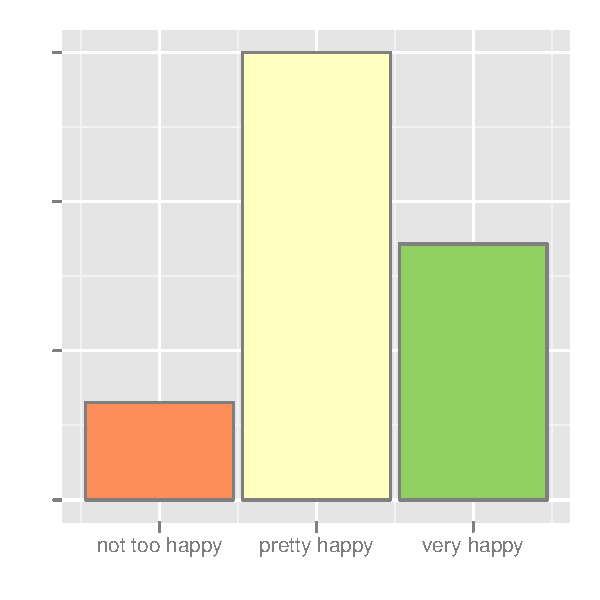
\includegraphics[width=0.33\linewidth]{part-hbar}%
  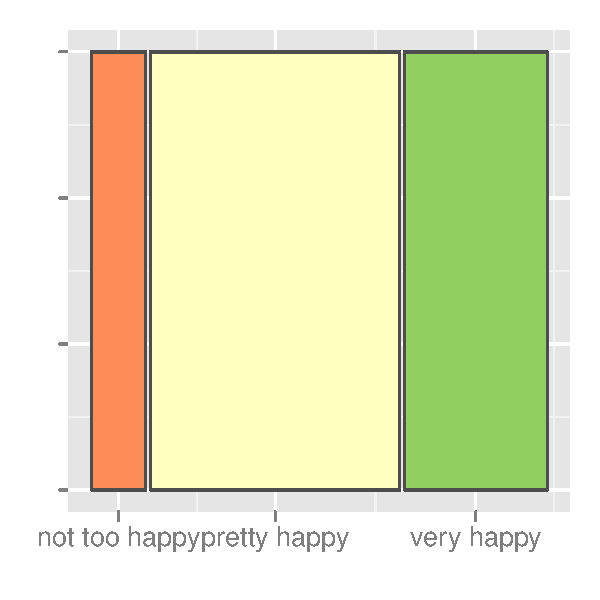
\includegraphics[width=0.33\linewidth]{part-hspine}%
  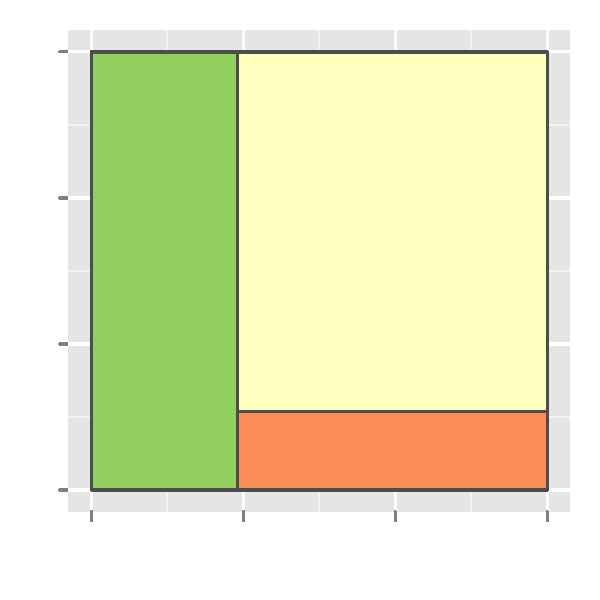
\includegraphics[width=0.33\linewidth]{part-treemap}

  \caption{1d partitions showing the distribution of happiness.  From left to right: bars, spines and tiles.}
  \label{fig:part-1d}
\end{figure}

\begin{itemize}
   \setlength{\itemsep}{0em}

  \item {\bf bar}s: height is proportional to value, width equally divides space. Bars are not space filling, occupying $\mbox{mean}(x - \max(x))$ of the total area. Bars can be arranged horizontally (``hbar'') or vertically (``vbar'').

  \item {\bf spine}s: width is proportional to value, height occupies full range. Spines are space filling and can be arranged horizontally (``hspine''), vertically (``vspine''), or can automatically pick their orientation (``spine'') by splitting the largest dimension. The name spine is evocative of books sitting on a library shelf \citep{hummel:1996}. Bars and spines are indistinguishable when the underlying data is evenly distributed across the categories.

  \item {\bf tile}s: no restrictions on height or width, just tile the plane with rectangles, trying to keep the aspect ratio of each rectangle close to 1. This is partitioning defined by the squarified treemap \citep{bruls:1999}.

\end{itemize}

Each of these three displays has different strengths and weaknesses. It is easiest to compare the value associated with bars because the perceptual task is the easiest: comparing position on a common scale. Reading spines and tiles are harder because we must compare lengths or areas, but they occupy the complete space and so work better recursively. 

We can create 2d primitives by combining these 1d primitives, as shown in Section~\ref{sec:combination}, but there is one 2d primitive that does not arise in this way.

\subsection{2d primitives}
\label{sub:part-2d}

2d primitives display 2d \emph{data}, i.e.\ a count broken down by two variables. We are currently aware of only one primitive for 2d data, the {\bf fluct}, derived from the fluctuation diagram \citep{hofmann:2000}. The fluct has height and width proportional to the square root of the count. Each rectangle is arranged on a regular grid formed by the levels of the two variables, allowing comparisons both vertically and horizontally.

A special case of the fluct is the equal bin size plot \citep{hofmann:2000} which occurs when the two variables are jointly uniformly distributed, usually as a result of the conditioning described in the following section. The equal bin size plot is particularly useful as a way of visualising missing combinations. Figure~\ref{fig:fluct} illustrates these two types of graphics.

\begin{figure}[htbp]
  \centering
  $f(age, marital)$
    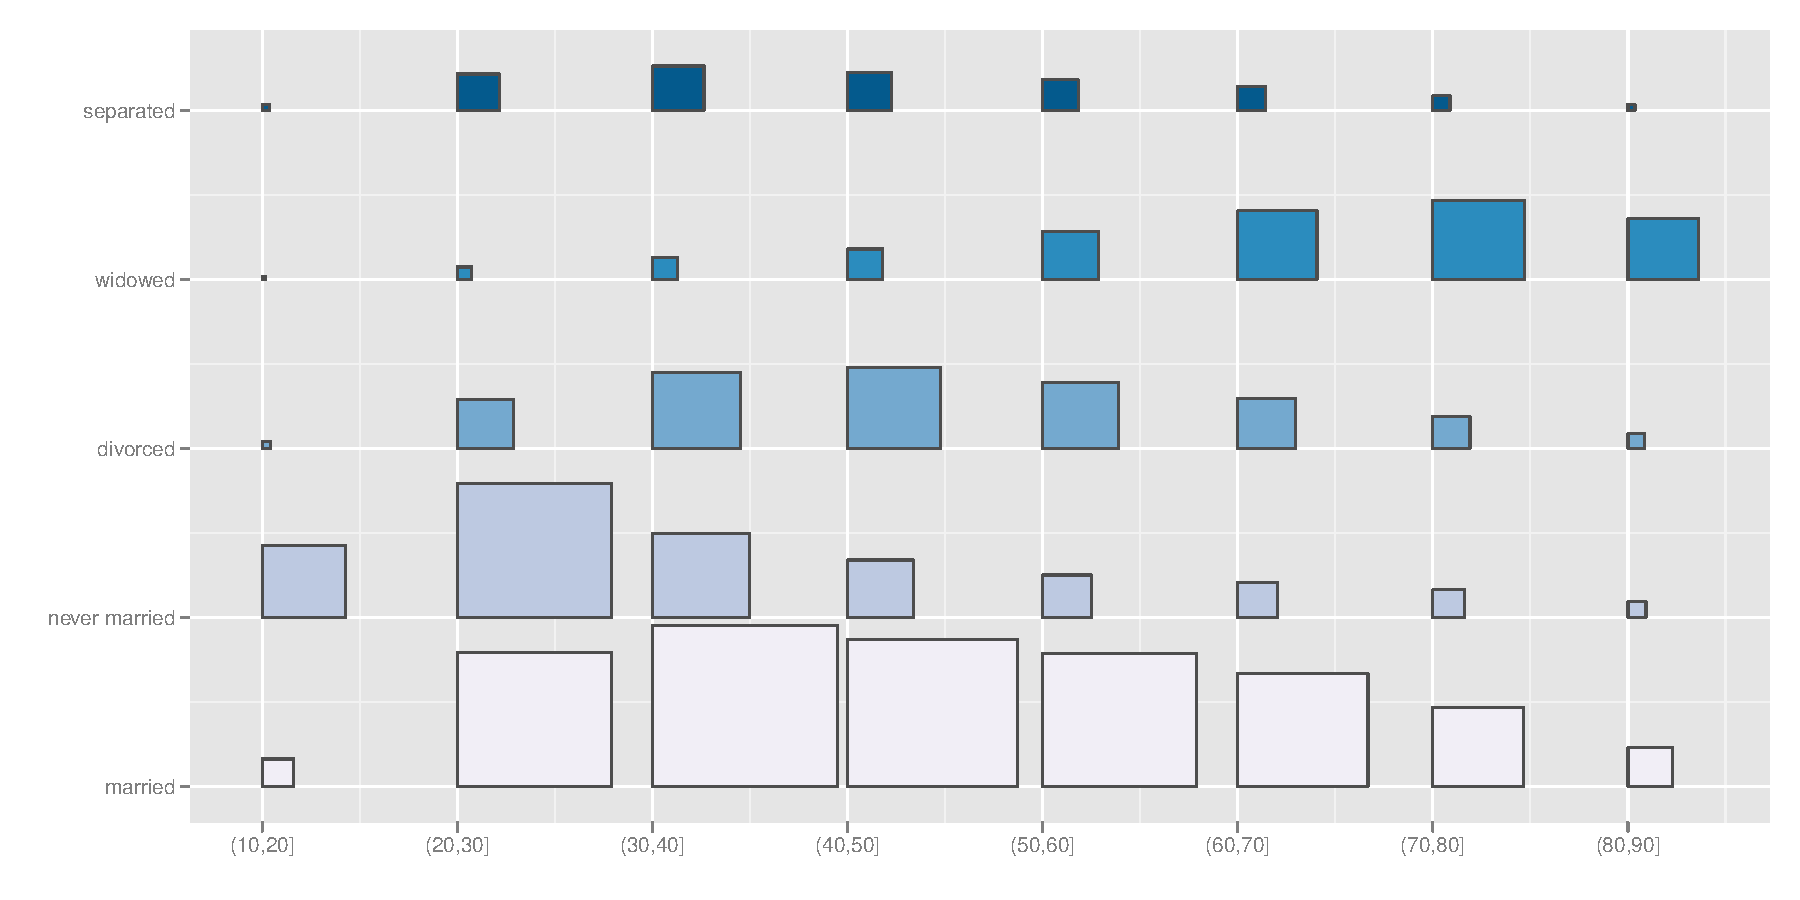
\includegraphics[width=0.9 \linewidth]{part-fluct}
  $f(1 | age, marital)$
    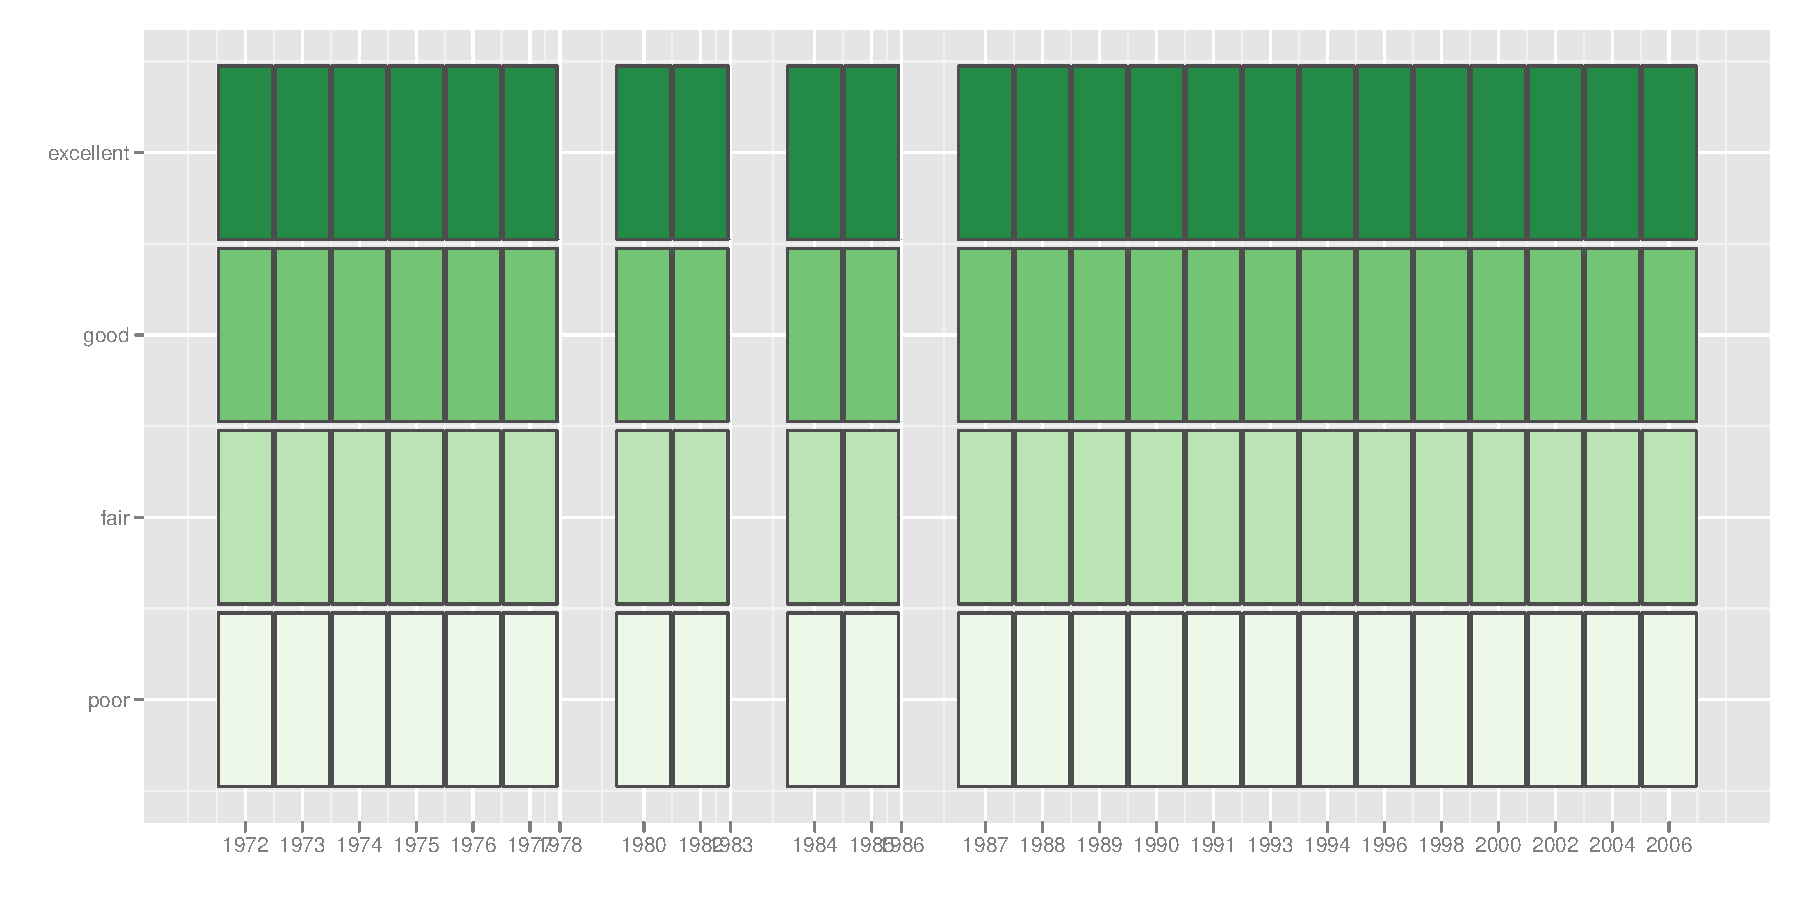
\includegraphics[width=0.9 \linewidth]{part-fluct-cond}
  \caption{(Top) A fluctuation diagram showing distribution of age (in decades) and marital status. (Bottom) Equal bin-size plot showing health status and survey year. Thee three empty columns show that health status was not recorded for three years.}
  \label{fig:fluct}
\end{figure}

\section{Probability and plot products}
\label{sec:combination}

To construct plots of higher-dimensional data sets, we need a way to decompose them into 1d and 2d components. Some statistical vocabulary is useful: one way of describing the input data is as a {\bf probability mass function}, or {\sc pmf}. A {\sc pmf} is a function with $n$ inputs, each indexing one dimension with an integer, and gives the probability of each combination of inputs. A {\sc pmf} has two restrictions: every value must be greater than or equal to zero, and all values must sum to one.  

\subsection{Joint distributions are the product of marginals and conditionals}

Figure~\ref{fig:2d-table} shows three ways to represent the the 2d table of proportions of sex and happiness. The top table displays the {\bf joint distribution}, and allows us to answer questions of the form ``what proportion of all people are male and very happy?'' The middle two tables displays two {\bf conditional distributions}: the distribution of sex given happiness, and happiness given sex. These correspond to restricting the row or column sums to one, and support questions such as ``what proportion of pretty happy people are female?'' or ``what proportion of males are not too happy?''. Finally, the last table displays the two {\bf marginal distributions} of sex and happiness. These allow us to answer questions like ``what proportion of respondents were male'' or ``what proportion of respondents were very happy?''.

\begin{figure}[ht]
  \begin{tabular*}{0.5\linewidth}{rrr}
\multicolumn{3}{l}{$f(happiness, sex)$}\\
  \toprule
  & male & female \\ 
  \midrule
  not too happy & 0.05 & 0.07 \\ 
  pretty happy & 0.25 & 0.31 \\ 
  very happy & 0.14 & 0.18 \\ 
  \bottomrule
  \end{tabular*}
  \\[1em]

 
  \begin{tabular*}{0.48\linewidth}{rrr}
\multicolumn{3}{l}{$f(happiness| sex)$}\\
  \toprule
  & male & female \\
  \midrule
  not too happy & 0.43 & 0.57 \\
  pretty happy & 0.45 & 0.55 \\ 
  very happy & 0.43 & 0.57 \\
  \bottomrule
  \end{tabular*}
%
\hspace{1em}
  \begin{tabular*}{0.48\linewidth}{rrr}
\multicolumn{3}{l}{ $f(sex|happiness)$}\\
  \toprule
  & male & female \\ 
  \midrule
  not too happy & 0.12 & 0.12 \\ 
  pretty happy & 0.57 & 0.55 \\ 
  very happy & 0.31 & 0.32 \\
  \bottomrule
  \end{tabular*}
  \\[1em]

  \begin{tabular}{rrrr}
\multicolumn{3}{l}{$f(happiness), f(sex)$}\\
  \toprule
  & male & female & \\ 
  \midrule
  not too happy & & & 0.12 \\ 
  pretty happy & & & 0.56 \\ 
  very happy & & & 0.30 \\
  & 0.44 & 0.56 \\ 
  \bottomrule
  \end{tabular}

  \caption{The distribution of happiness and sex, displayed in three equivalent ways.  (Top) Joint distribution. Overall table sums to one. (Middle) Conditional distribution of sex given happiness and marginal distribution of happiness. (Bottom) Conditional distribution of happiness given sex and marginal distribution of sex.}
  \label{fig:2d-table}
\end{figure}

Formally, a conditional distribution function is written $f(x | y)$ and is equal to $f(x, y) / f(y)$. This definition illustrates that an important statistical fact: given a conditional distribution and a marginal distribution, we can always find the joint distribution: $f(x, y) = f(x | y)\,f(y)$ \footnotemark. This definition extends in a straightforward way to higher dimensions. For example, a 3d joint distribution can be written as the product of 2d and 1d conditional and marginal distributions in the following three ways:

\begin{itemize}
  \setlength{\itemsep}{0em}
  \item $f(x, y, z) = f(z)\,f(x, y | z)$
  \item $f(x, y, z) = f(y, z)\,f(x | y, z) $
  \item $f(x, y, z) = f(z)\,f(y | z)\,f(x | y, z)$
\end{itemize}

\footnotetext{Because the parameters of a {\sc pmf} identify it, statisticians often fail to explicitly label the different functions. To be precise, the above statement should be written: $f_{X, Y}(x, y) = f_{X|Y=y}(x | y)\,f_Y(y)$}

This means that we can turn any high-dimensional {\sc pmf} into a product of low-dimensional conditional and marginal {\sc pmf}s, a computationally trivial operation. It remains to find a graphical analog of this multiplication. 

\subsection{Area is the product of height and width}

We connect probability products to our rectangular primitives by noting that areas are also products: products of height and width. It's easiest to show this with a picture: Figure~\ref{fig:fact-simple} shows how our simple 1d primitives combine to get two familiar plots: the mosaic plot and the stacked bar chart. From left to right, we have plots of $f(happy)$, $f(sex | happy)$ and the product $f(happy, sex)$. The heights and widths of the rectangles are multiplied in the same way as the components of the {\sc pmf}.

\begin{figure}[htbp]
  \centering
  \includegraphicsinline{0.3\linewidth}{fact-happy} = %
  \includegraphicsinline{0.3\linewidth}{fact-happy|sex} = %
  \includegraphicsinline{0.3\linewidth}{fact-happy-sex}

  \includegraphicsinline{0.3\linewidth}{fact-happy-2} $\times$ %
  \includegraphicsinline{0.3\linewidth}{fact-happy|sex-2} = %
  \includegraphicsinline{0.3\linewidth}{fact-happy-sex-2}

  \caption{Plots of the distribution of happiness and sex (\key{male} male, \key{female} female) (Left) $f(happy)$, (Middle) $f(sex | happy)$, (Right) $f(happy, sex)$.}
  \label{fig:fact-simple}
\end{figure}

Figure \ref{fig:recursive} shows a more complicated example: visualising a 3d distribution as a product of three low-dimensional distributions. We first display $f(marital)$, then $f(marital, sex) = f(sex | marital) f(marital)$, and finally $f(marital, sex, happy) = f(happy | sex, marital) f(sex | marital) f(marital)$. This plot uses two vspines and an hspine to produce a mosaic plot.

\begin{figure}[htbp]
\begin{minipage}[b]{0.3\linewidth}
  	$f(marital)$
      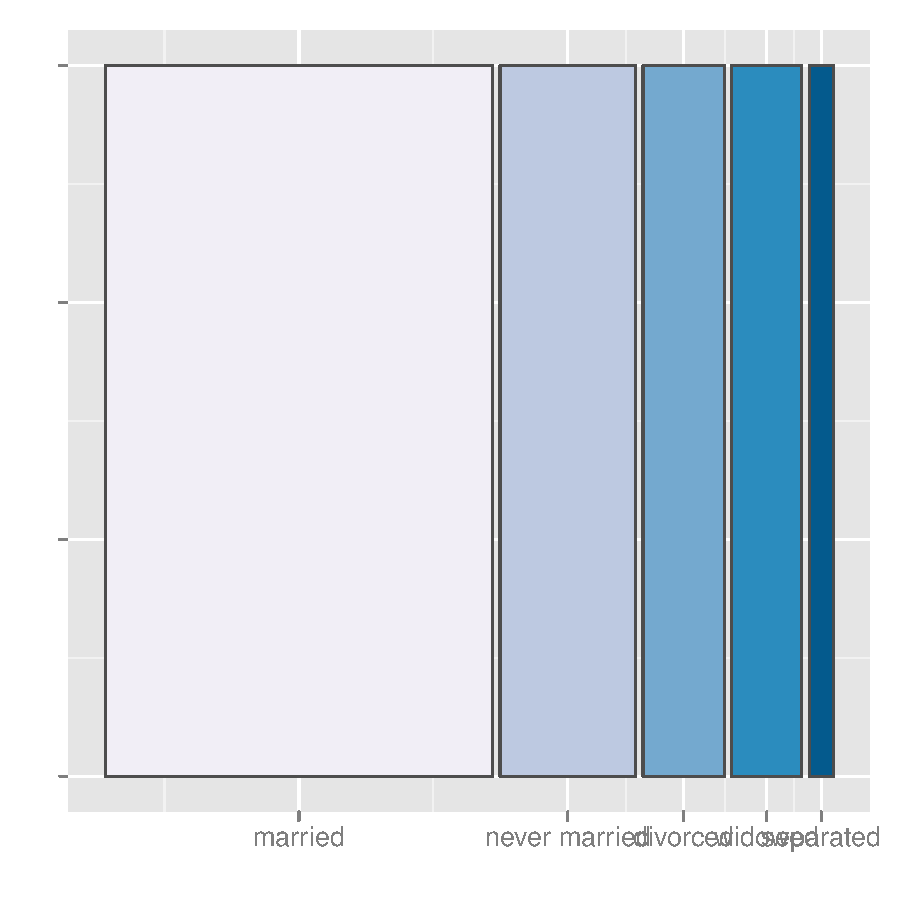
\includegraphics[width=\linewidth]{part-comb-1}%
\end{minipage} 
\begin{minipage}[b]{0.3\linewidth}
$f(marital, sex)$ 
       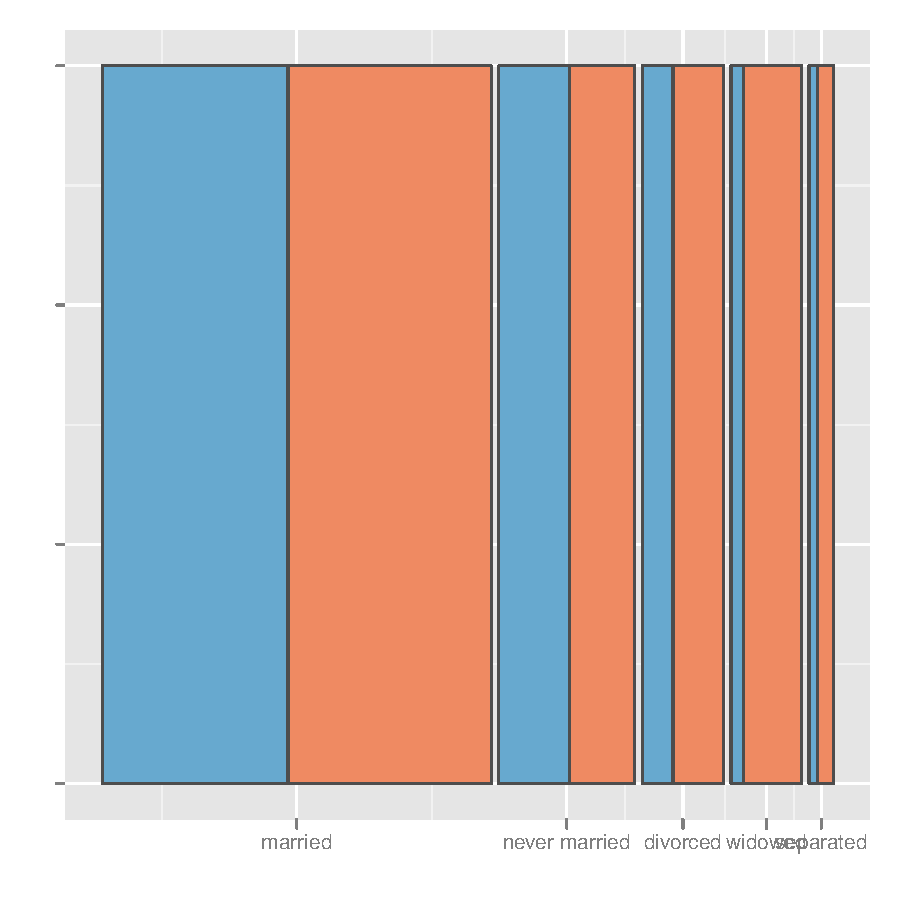
\includegraphics[width=\linewidth]{part-comb-2}
\end{minipage} 
\begin{minipage}[b]{0.3\linewidth}
$f(happy, sex, marital) =$
$f(happy|marital, sex) \cdot $
$f(marital, sex)$
      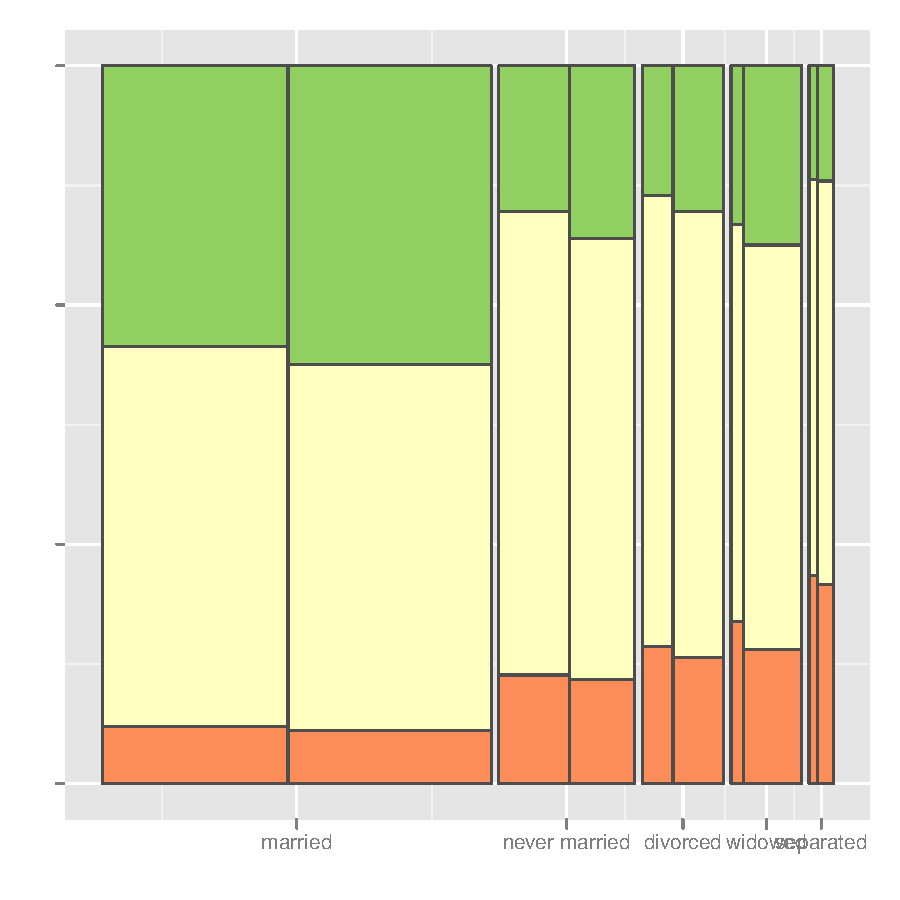
\includegraphics[width=\linewidth]{part-comb-3}
\end{minipage}
  \caption{Conditional on marital status, are men or women happier?  This figure shows the construction of $f(happy, sex, marital)$ with (from left to right) a vspine by marital status, a vspine by marital status and sex, and a hspine by marital status, sex and happiness.  For all levels of marital status, men are slightly less happy.}
  \label{fig:recursive}
\end{figure}

   
More precisely, a product plot is constructed by the following recursive partitioning algorithm, which takes three parameters: {\sf data}, a multi-dimensional array, with dimensions ordered in the same way as the desired partitions; {\sf bounds}, a vector giving the top, left, right and bottom boundaries; and {\sf divider}, a list of the desired low-d drawing primitives. The following algorithm gives an rough idea of the computation:

\begin{itemize}
  \item Calculate the one marginal and $i$ conditional distributions.

  \item For each probability in the marginal distribution, divide the current bounds into $i$ sets of new bounds, one for each level of the categorical variable. The new bounds are found using the algorithm defined by the drawing primitive.

  \item For each new bound and matching conditional distribution, call the partition function recursively, dropping one element from the list of drawing primitives.

\end{itemize}

Different partitions reveal different features of the data. Take for example, the distribution of age and marital status, as shown in Figure~\ref{fig:fluct}. Instead of visualising the joint distribution with a fluct, we could focus on the conditional distribution of marital status given age, or age given marital status. Figure~\ref{fig:marital} shows two ways to do this. The left plot shows $f(marital, age)$ with a vspine nested in a hspine, and the right plots $f(age, marital)$ with a hbar nested in a vspine. These displays show the same data, but support different comparisons: on the left, we can see that most young people are unmarried, and on the right, that few unmarried people are over the age of 30. The right plot, with bars nested inside spines, also illustrates an important feature of non-space filling tilings: the relationship between proportion and area is only constant within a level. The bars are scaled to be as tall as possible, without overflowing any bounding region.

\begin{figure}[htbp]
  \centering
$f(marital, age) =$\\
\begin{minipage}[t]{0.49\linewidth}
\centering 
$f(marital|age)f(age)$ 
    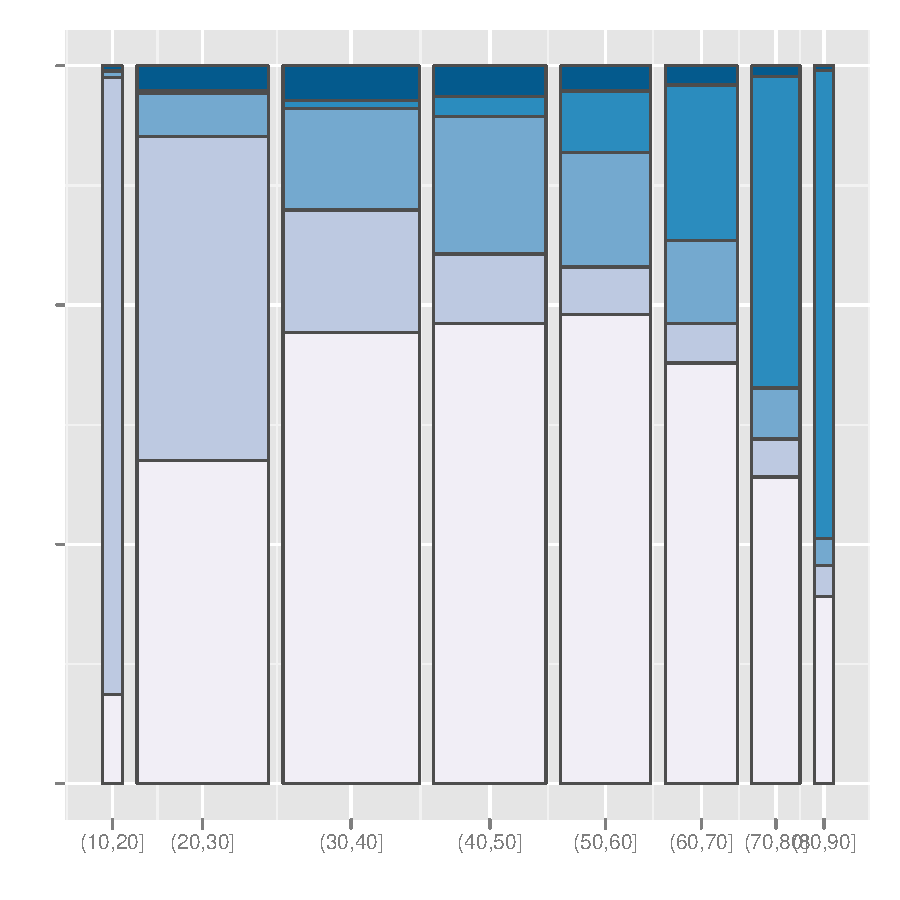
\includegraphics[width=\linewidth]{part-marital-1}%
 \end{minipage}
\begin{minipage}[t]{0.49\linewidth}
\centering
 $f(age|marital)f(marital)$
    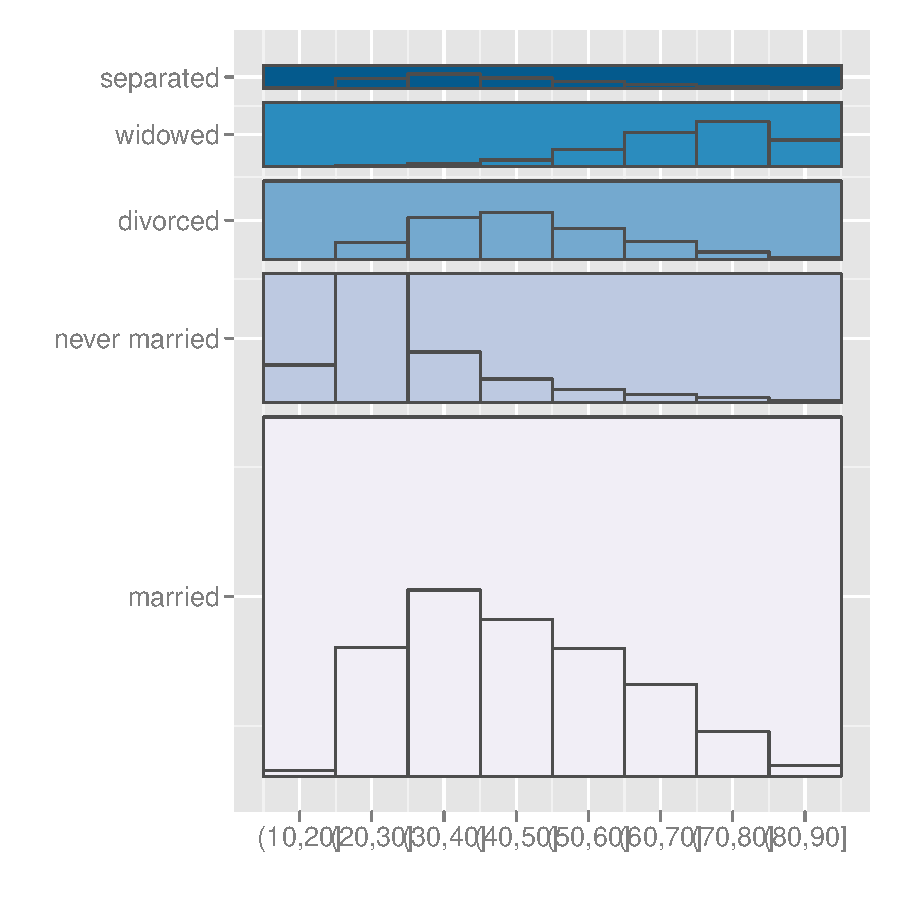
\includegraphics[width=\linewidth]{part-marital-2}
 \end{minipage}
  \caption{(Left) The joint distribution of marital status and age, $f(marital, age)$ as $f(marital|age) \cdot f(age)$, (in decades) partitioned by a vspine and hspine.  (Right) The joint distribution of age and marital status, $f(age, marital)$, partitioned by a vspine and hbar.}
  \label{fig:marital}
\end{figure}

Conditioning is also an important tool by itself, because it allows one to remove relationships that are known or uninteresting. Figure~\ref{fig:part-cond} uses a fluct and a vspine to explore the relationship between happiness, health and financial status. The left plot displays raw proportions, showing that most people are in good health and average financial standing. However, it is difficult to see how happiness varies within these conditions because we must compare areas, not positions. Conditioning on financial status and health produces the plots on the right (equal bin size plots) and makes it easier to see the conditional distribution of happiness given sex and health, because comparing positions along a common scale is an easier perceptual task. Depending on the comparison we are most interested in, we can make it easier to compare across wealth given health, or health given wealth. Here we see that for a fixed income level, better health is correlated to increased happiness. The same is not true for a fixed level of health: rich people with poor health seem to be less happy than poorer people in poor health.

\begin{figure*}[htbp]
  \centering
\begin{minipage}[b]{0.32\linewidth}
\centering
$f(happy, health, finrela) =$
$f(happy | health, finrela) \times f(health, finrela)  $
     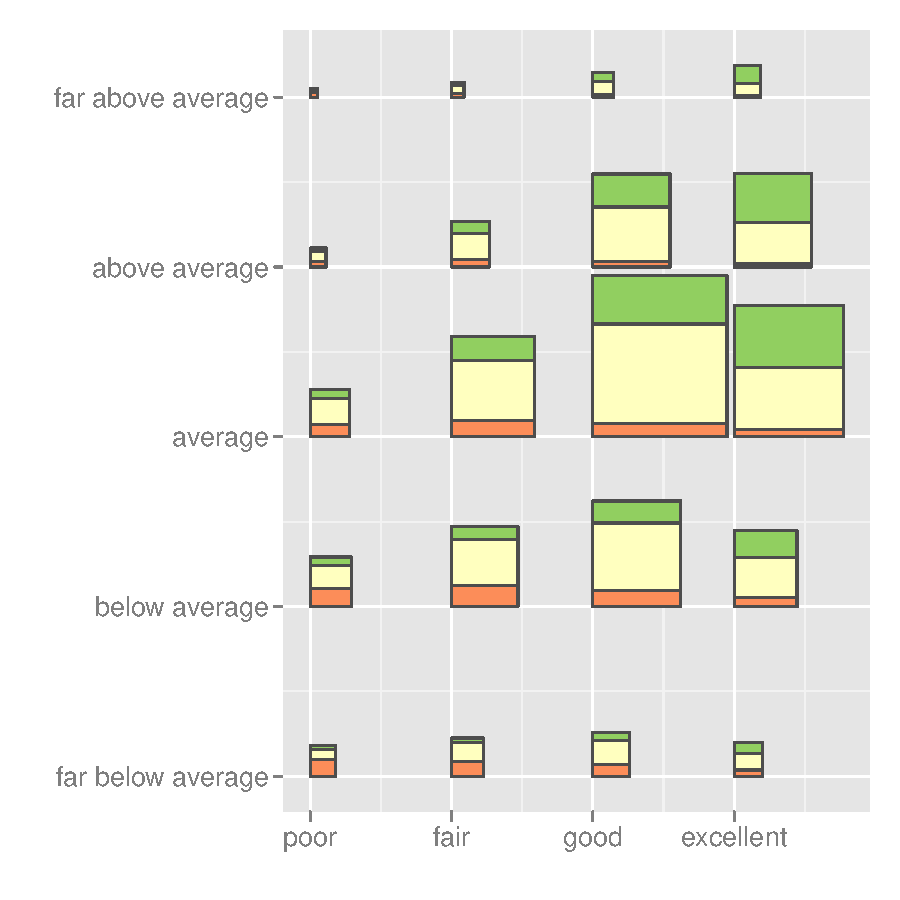
\includegraphics[width=\linewidth]{part-fluctuation}
 \end{minipage}
%
\begin{minipage}[b]{0.32\linewidth}
\centering
$f(happy | health, finrela)$
    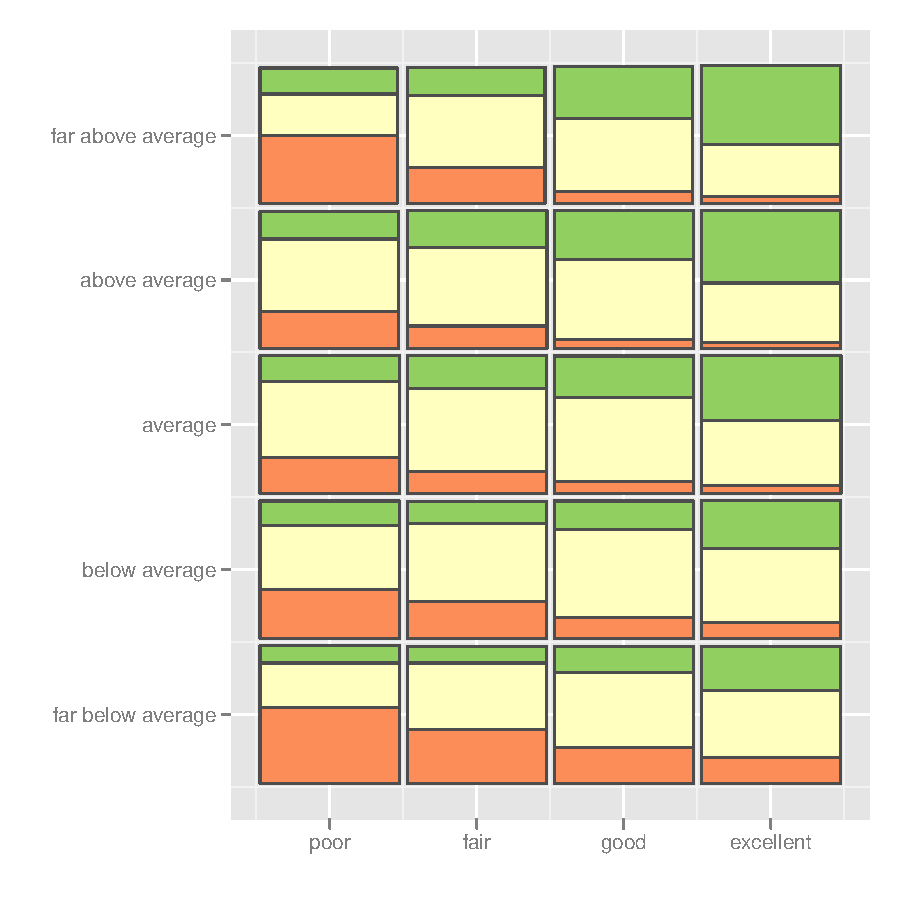
\includegraphics[width=\linewidth]{part-equal-area}
 \end{minipage}
%
\begin{minipage}[b]{0.32\linewidth}
\centering
$f(happy | health, finrela)$
    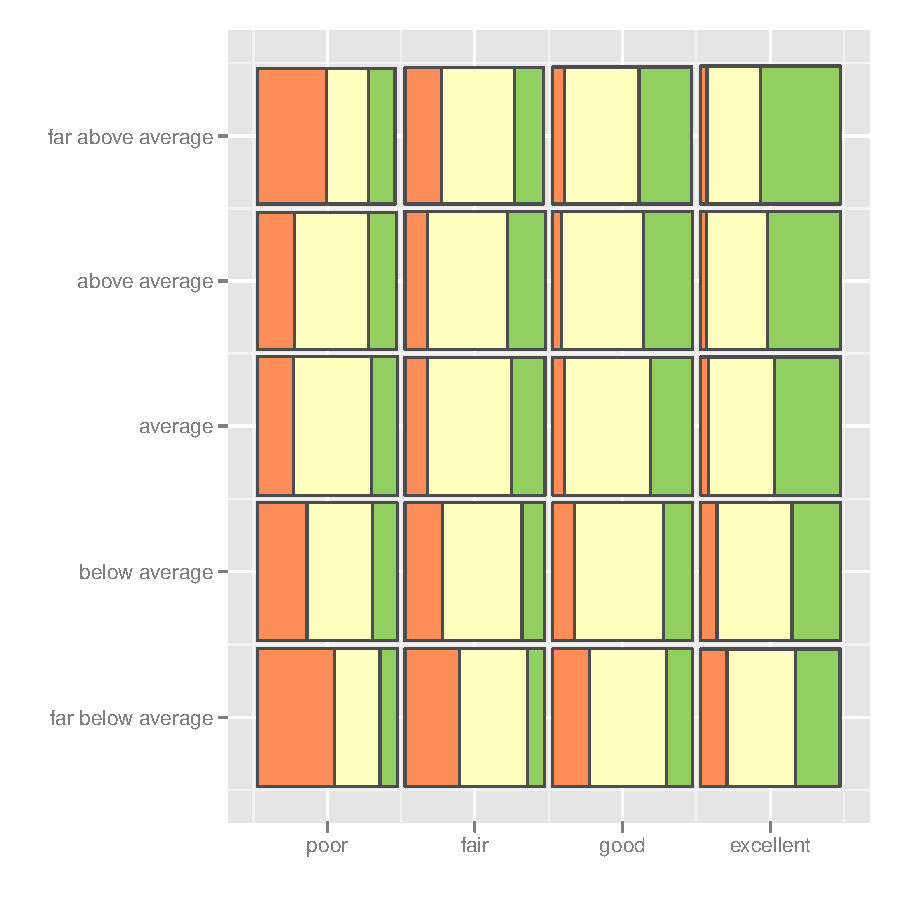
\includegraphics[width=\linewidth]{part-equal-area-2}
 \end{minipage}
%
    %
    
  \caption{(Left) $f(happy, health, finrela) = f(happy | health, finrela) \times f(health, finrela)  $, partitioned with a vspine and fluct.  Health is on the $x$-axis, financial status on the $y$-axis. (Middle) $f(happy | health, finrela)$. We can no longer see the joint distribution of health and financial status, but it is much easier to see the conditional distribution of happiness. Healthier and richer people are happier: maybe money does buy happiness? (Right) $f(happy | health, finrela)$ partitioned with a fluct and {\bf h}spine. (\key{not-too-happy} Not too happy, \key{pretty-happy} pretty happy, \key{very-happy} very happy)}
  \label{fig:part-cond}
\end{figure*}

\section{Existing plot types}
\label{sec:existing}

Many existing plots fall into this framework. The low-d primitives already have their own names:

\begin{itemize}
  \setlength{\itemsep}{0em}
  \item {\bf Bar chart} (1d). 1 hbar.
  \item {\bf Column chart} (1d). 1 vbar.
  \item {\bf Spineplot} (1d). 1 spine.
  \item {\bf Fluctuation} diagram (2d): 1 fluct.
\end{itemize}

\noindent And many more plots correspond to higher order combinations:

\begin{itemize}
  \setlength{\itemsep}{0em}
  
  \item {\bf Stacked} bar chart (2d). $1$ hbar and $1$ vspine.

  \item {\bf Nested} bar chart \citep{peltier:2009} (2d). $2$ hbars. 

  \item {\bf Equal bin size} plot \citep{hofmann:2000} (3d): $1$ fluct and $1$ vspine, conditioned on the first two variables.

  \item {\bf Mosaic} plot \citep{hartigan:1981,friendly:1994,hofmann:2003} (nd). Alternating hspines and vspines. 

  \item {\bf Double-decker} plot \citep{hofmann:2001} (nd). $n-1$ hspines and $1$ vspine. 

  \item {\bf Treemap} \citep{shneiderman:1992} (nd): $n$ spines.

  \item {\bf Squarified treemap} \citep{bruls:1999} (nd): $n$ tiles.

  \item {\bf Generalised treemaps} \citep{vliegen:2006} (nd): any plot ending with a tile.

\end{itemize}

Trellis graphics \citep{becker:1996}, also known as latticed, facetted and conditioned graphics, are another related display. They use categorical variables to generate multiple panels, each containing a plot of the subset of the data. Trellised plots of area graphics also fall into our framework and can be created by conditioning on the trellising variables.

\section{Display considerations}
\label{sec:display}

Labelling product plots is challenging. In this paper, we use a carefully selected combination of colour and axis labels, as well displaying the process by which a product plot is created. Axis labels are only available under certain conditions: when we have rows or columns that all share the same dimensional index. This can occur because of the structure of the graphical primitive (e.g. bars, flucts), or because the display is of a conditional distribution. Take Figure~\ref{fig:marital} for example: the left plot can only have the $x$ axis labelled, but the right plot can have both axes labelled. There are other ways to label the cells apart from colour. \citep{slingsby:2009} uses text labels, sized to occupy the space of the region they label. In the interactive setting, dynamic labelling in the form of tool tips is extremely helpful, as is the ability to use linked brushing to connect high-d plots to low-d plots.

We have observed that some aspect ratios are more aesthetically pleasing than others. This is particularly obvious for the fluctuation diagram where, in our experience, the plots are most appealing when the flucts are square. In other plots there does not seem to be an easy rule of thumb, but we wonder if aspect ratios close to the golden ratio might be more appealing. We are not aware of any previous work on aesthetics of aspect ratio, although they do seem to affect perception \citep{kong:2010}. More research in this area is needed, particularly to explore the balance of aesthetics and usability.


\section{Variations and extensions}
\label{sec:variations}

On top of this basic framework, it is useful to consider a few variations and extensions. Instead of counts, we can plot weighted data or continuous data, or we can relax the display constraints to allow displays where area is not proportional to weight, partitions are non-disjoint or non-rectangular.

\subsection{Weighting}
\label{sub:weighting}

We have assumed that the proportions represent counts, but without loss of generality, we can use any set of non-negative, additive weights. For example, in the happy dataset, the {\sf wtssall} variable gives analytic survey weights. These are used to account for oversampling of black respondents in certain years, and to reduce the effect of non-response in other demographics. Figure~\ref{fig:weighting} shows the difference between the weighted and unweighted distributions of age and sex. The distribution is barely different, and suggests that we don't need to worry about weights for this plot. (Unfortunately for this dataset of we have been unable to find any plots where weighting does makes a difference.)  In other datasets, weights can be useful to move from numbers of counties to numbers of people, or to areas, or to other relevant quantities. Some examples of weighted data graphics can be found in \citep{unwin:1998,unwin:2003aa,unwin:2006}.

\begin{figure}[htbp]
  \centering
    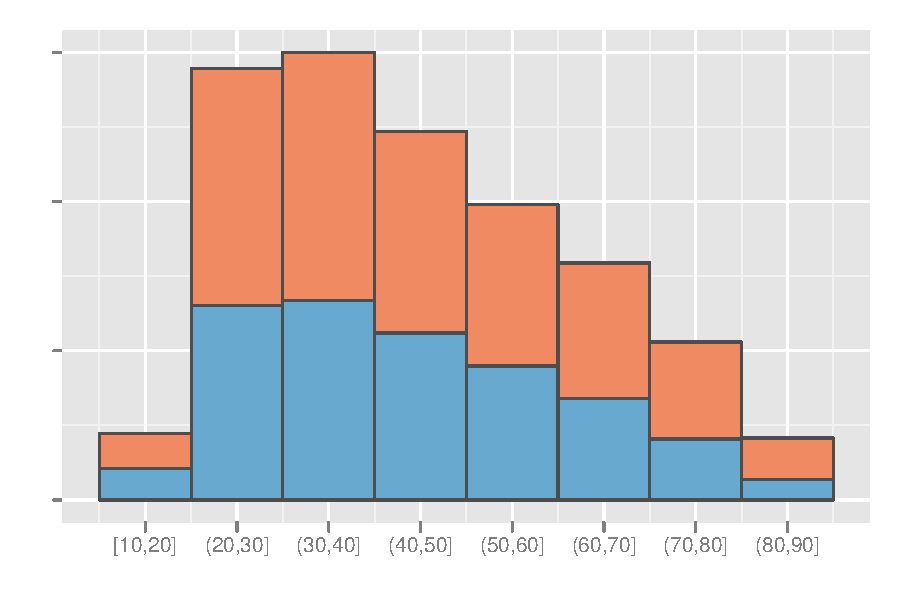
\includegraphics[width=0.5\linewidth]{wt-count}%
    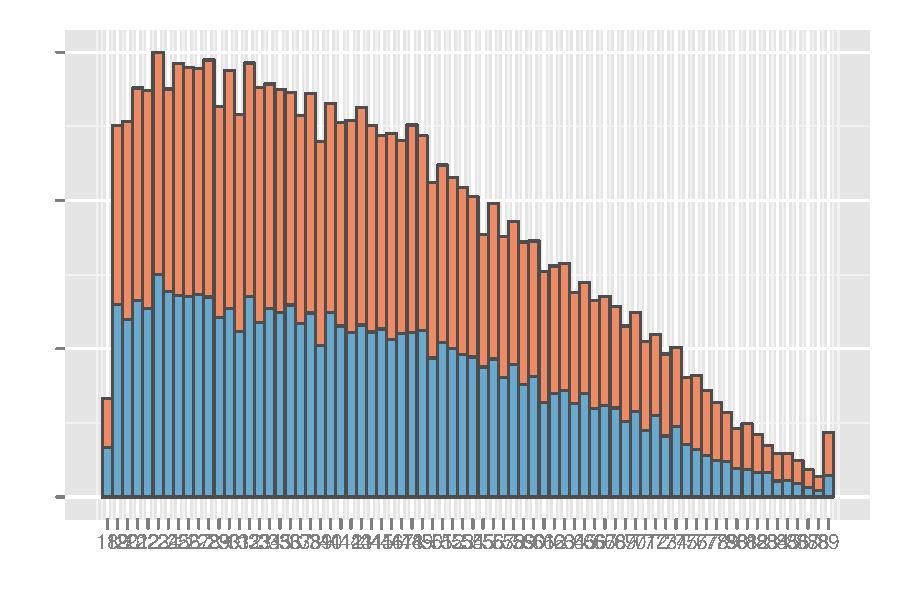
\includegraphics[width=0.5\linewidth]{wt-wtssall}%
  \caption{Joint distribution of age and sex (\key{male} male, \key{female} female), $f(age, sex)$. (Left) counts and (right) probability weights. In this case, there is very little difference between the plots.}
  \label{fig:weighting}
\end{figure}

\subsection{Continuous data}
\label{sub:continuous_data}

The framework can be trivially extended to work with continuous data: just  bin continuous variables to make them discrete. There are many different to ways to create bins for continuous data, but two are most important \citep{denby:2009}: bins of equal width, and bins containing equal numbers of points. This extension allows the product plot framework to also describe {\bf histograms} and {\bf spinograms} \citep{hummel:1996}, continuous analogues of bar and spine charts, shown in Figure \ref{fig:cont-examples}. A long standing tradition is that no gaps are displayed between adjacent rectangles when displaying continuous data. 

A more theoretical approach in dealing with continuous variables  lies in increasing the number of bins infinitesimally -- this leads from a probability mass function to a density function, making the 1d primitives of hbar and vbar to density plots, and changing the spine-plot representation to a conditional density plot (citation needed - probably Martin's and Heike's paper). While the inclusion of one continuous variable is completely feasible that way, two variables need the use of an additional aesthetic, such a s colour,  to visualize a 2d joint density. Three or more continuous variables break the scope of the product plots framework.

\begin{figure}[htbp]
  \centering
  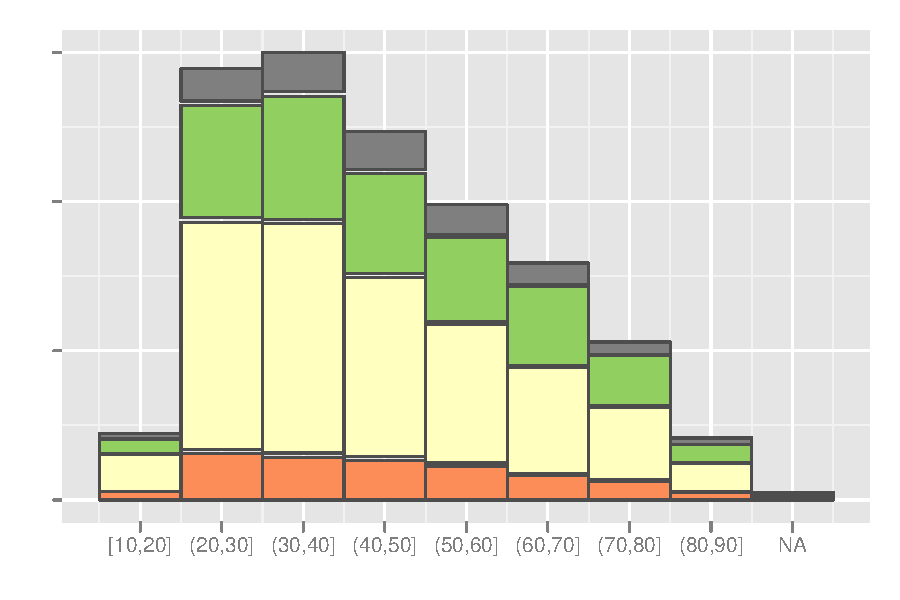
\includegraphics[width=0.5\linewidth]{cont-hbar}%
  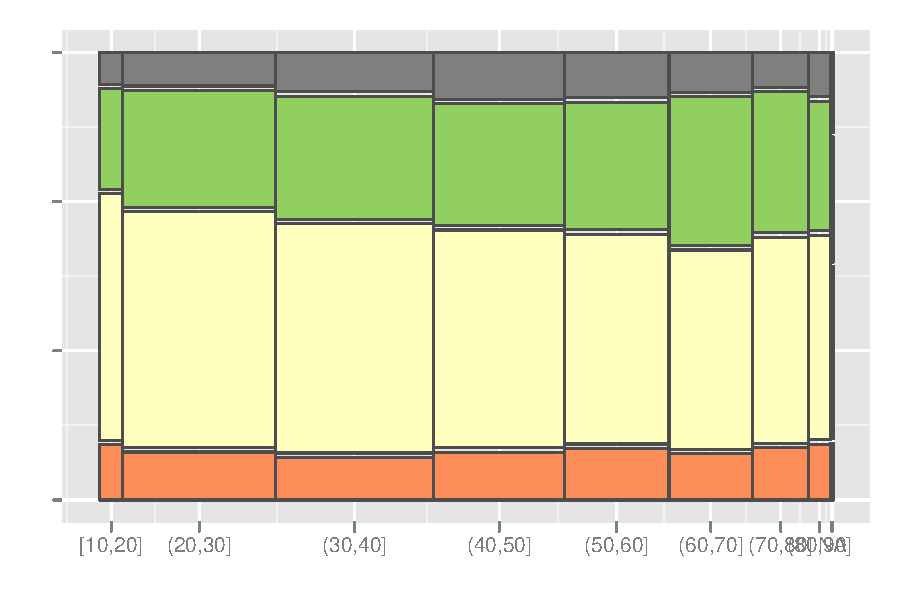
\includegraphics[width=0.5\linewidth]{cont-hspine}
  
  \caption{The distribution of happiness with age, $f(age, happy)$. (Left) hbar + vspine: an extension of the histogram. (Right) hspine + vspine: an extension of the spinogram.}
  \label{fig:cont-examples}
\end{figure}

With one more extension, displaying the innermost proportion with colour (instead of area), we can also describe {\bf dimensional stacking} \citep{leblanc:1990}.

\subsection{Area not proportional to weight}

It can be useful to violate the constraint that area is proportional to value to distinguish between zeros, missing values and very small values. A zero weight should have zero area, but giving it positive area can be useful so that it is visible. In general, it's useful to constrain all areas to be above a certain minimal perceptible size (e.g.\ 4 square pixels). Areas which are constrained in such a way need a visual flag (such as a different colour) to ensure that the reader knows that the relationship between area and value has been violated. This type of non-linear mapping has been implemented in {\sc manet} \citep{unwin:1996} and in hierarchical pixel bar charts \citep{keim:2002}. At the other end of the spectrum, it can be useful to constrain the size of largest values to get censored zooming \citetext{Antony Unwin, priv. comm.}, which makes it possible to focus on small values.

Other non-linear transformations may also be useful. For example, we could take square roots to stabilise the variance of the areas. Tukey applied this technique to histograms to create rootograms \citep{wainer:1974,tukey:1971}: histograms where the y-axis has a square root scale.

\subsection{Non-disjoint partitions}

Cascaded treemaps \citep{lu:2008} illustrate how the violation of containment can be productive. In the {\bf cascaded treemap}, each level is slightly offset from the one above to create a pseudo-3d perspective. This makes it easier to see all the levels of the hierarchy, not just the lowest level. Figure~\ref{fig:cascade} shows an example of how cascading can help illuminate the structure of a complex mosaic plot. This technique is probably most effective when implemented interactively.

\begin{figure}[htbp]
  \centering
    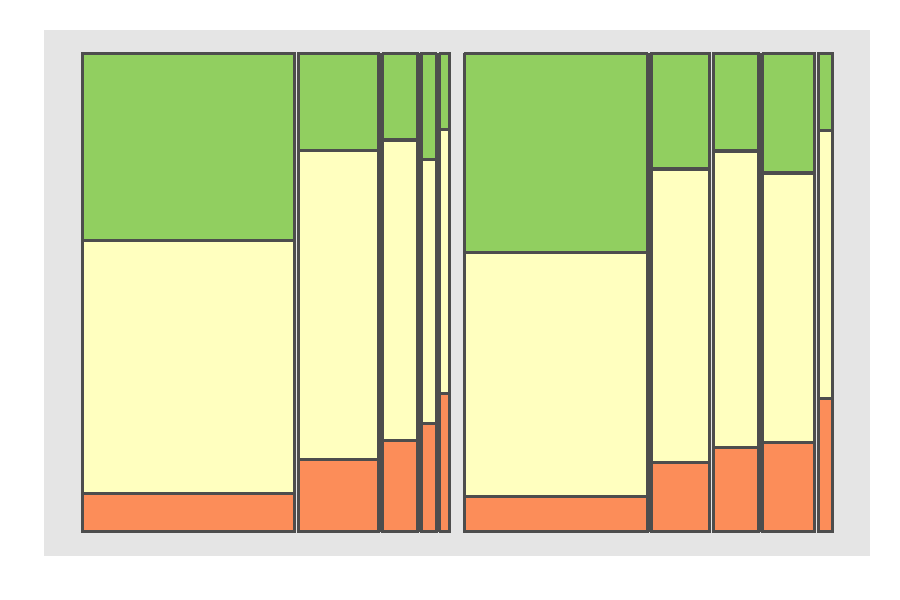
\includegraphics[width=0.5\linewidth]{sex-marital-happy}%
    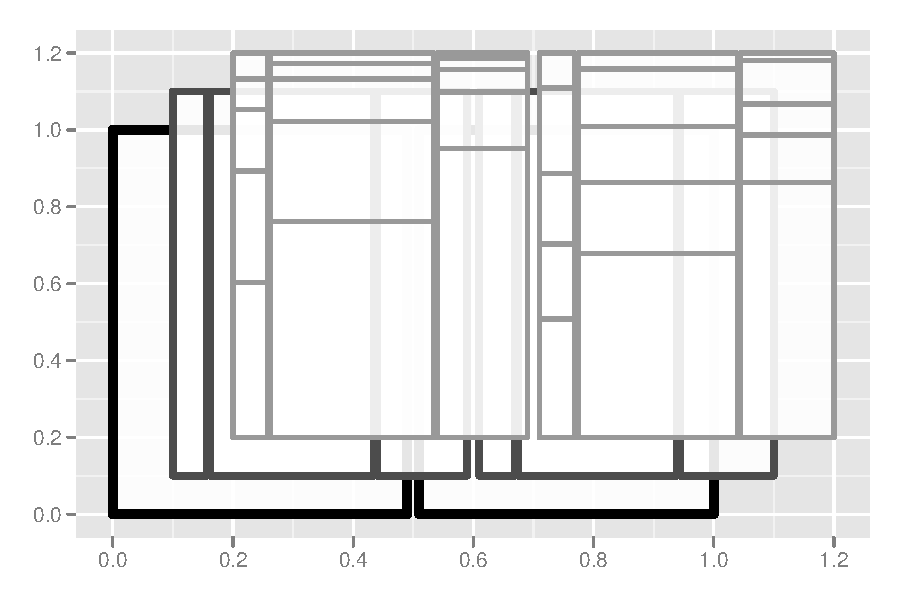
\includegraphics[width=0.5\linewidth]{cascade}
  \caption{A mosaic plot of happiness by marital status and sex, $f(happy, marital, sex)$. (Left) Coloured by happiness (\key{not-too-happy} Not too happy, \key{pretty-happy} pretty happy, \key{very-happy} very happy).  (Right) A cascaded view helps show how the plot is built up.}
  \label{fig:cascade}
\end{figure}

\subsection{Non-rectangular partitions}

A pie chart is a popular method of displaying proportions, but it is not a rectangular partition and so does not seem to fall in the framework of this paper. However, there is a simple relationship between product plots and pie charts: a pie chart is an hspine drawn in polar coordinates with the $x$ coordinate mapped to angle and the $y$ coordinate to radius. Many other circular displays turn out to be special cases of product plots drawn in polar coordinates \citep{draper:2009}. We have identified the following radial plots as polar transformations of product plots:

\begin{itemize}
  \setlength{\itemsep}{0em}
  
  \item {\bf Wind rose} (aka sector graphic) \citep{lalanne:1843} and {\bf fourfold displays} \citep{friendly:1995} (2d): 1 hbar, and 1 vspine. Nightingales's coxcomb \citep{nightingale:1857} is very similar, but the slices overlap and so violate the constraint of disjoint area.

  \item {\bf Concentric pie chart} (aka bullseye chart) (1d): 1 hspine.

  \item {\bf Doughnut plot} (2d): 1 hspine, and 1 vspine.

  \item {\bf Racetrack plot} (aka circular bar chart) (1d): 1 vbar.

  \item {\bf Infoslices} \citep{andrews:1998} (nd): $n$ vbars. But they only use half of the polar plane, and are specialised for highly nested data.

\end{itemize}

\noindent Eight polar variants are displayed in Figure~\ref{fig:polar}. Many of these are familiar and already have names. They are all of dubious utility because research suggests that visualisations in polar coordinates are harder to reader accurately than visualisations in Cartesian coordinates \citep{diehl:2010}.

Generally, the y axis (mapped to radius) must be square-root transformed to ensure that that counts stay proportional to areas. Fan-lenses \citep{lou:2007} and Stasko's radial displays \citep{stasko:2000} deliberately do not do this in order to emphasise the outer levels.

\begin{figure}[htbp]
  \centering
    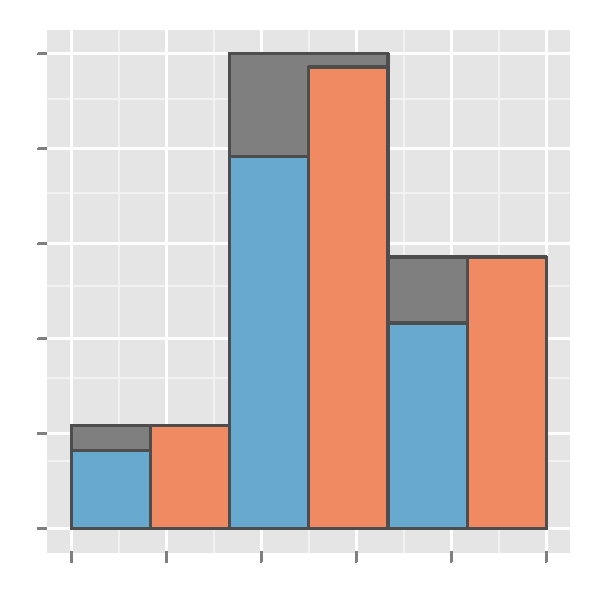
\includegraphics[width=0.25\linewidth]{hb-vb-cartesian}%
    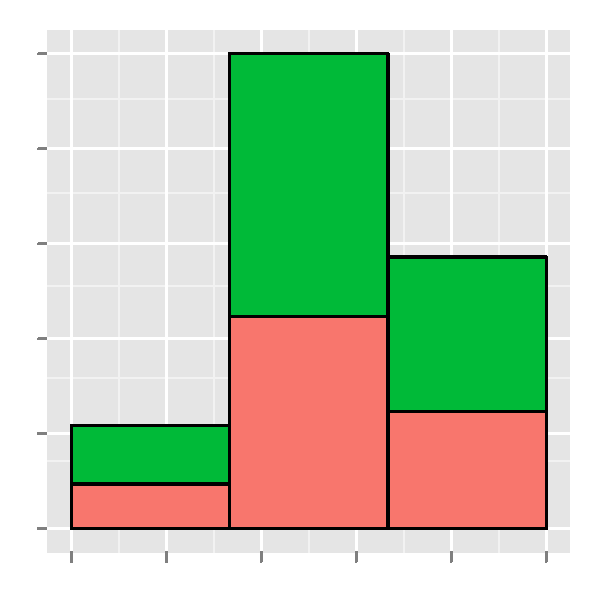
\includegraphics[width=0.25\linewidth]{hb-vs-cartesian}%
    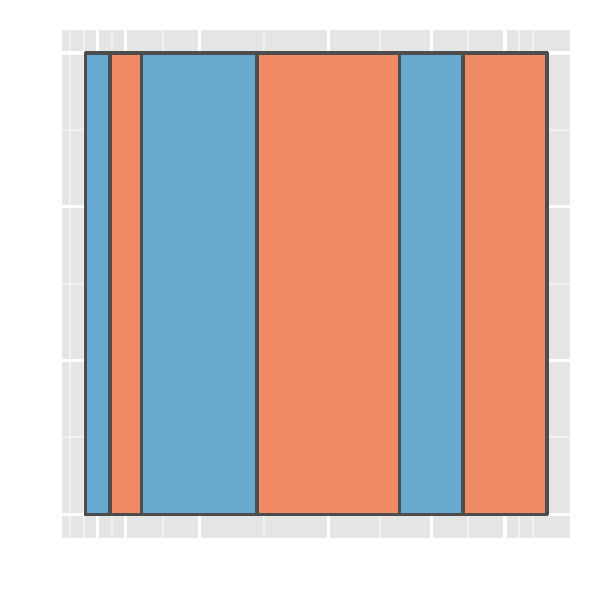
\includegraphics[width=0.25\linewidth]{hs-hs-cartesian}%
    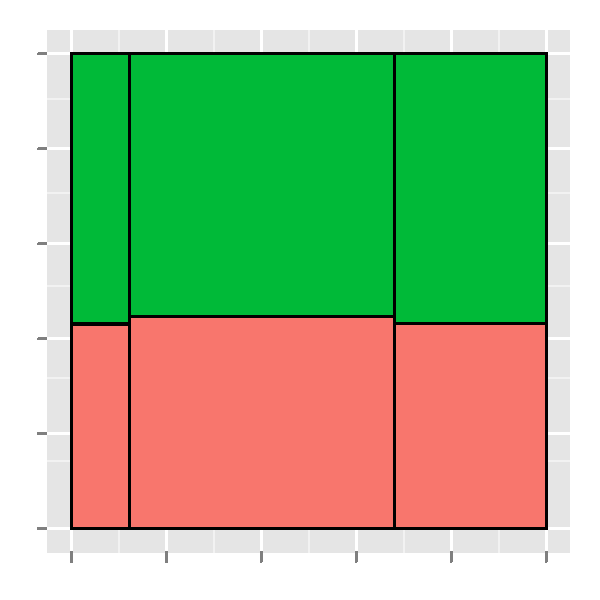
\includegraphics[width=0.25\linewidth]{hs-vs-cartesian}

    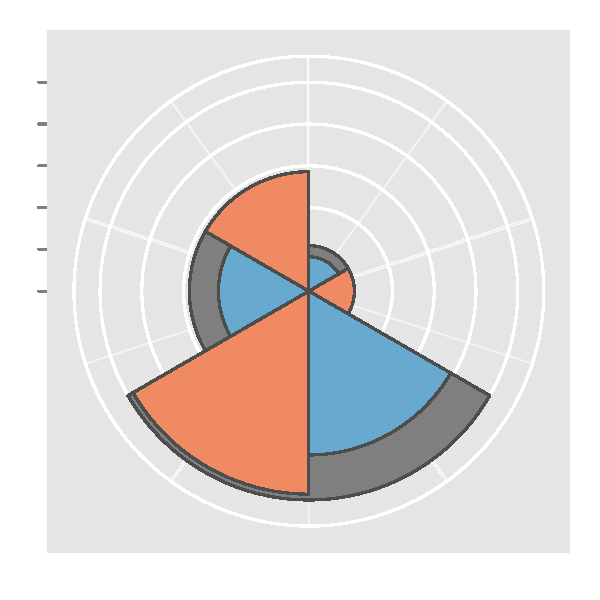
\includegraphics[width=0.25\linewidth]{hb-vb-polar}%
    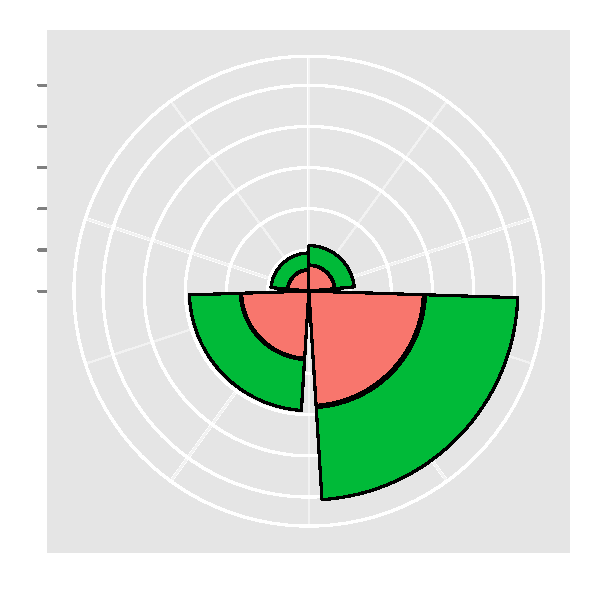
\includegraphics[width=0.25\linewidth]{hb-vs-polar}%
    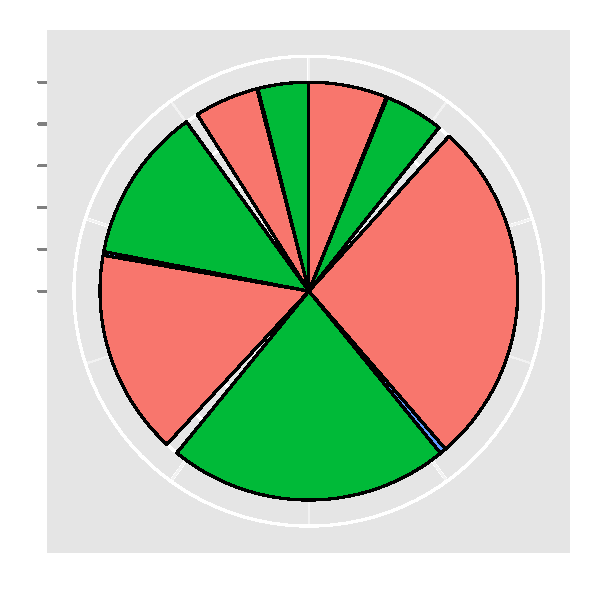
\includegraphics[width=0.25\linewidth]{hs-hs-polar}%
    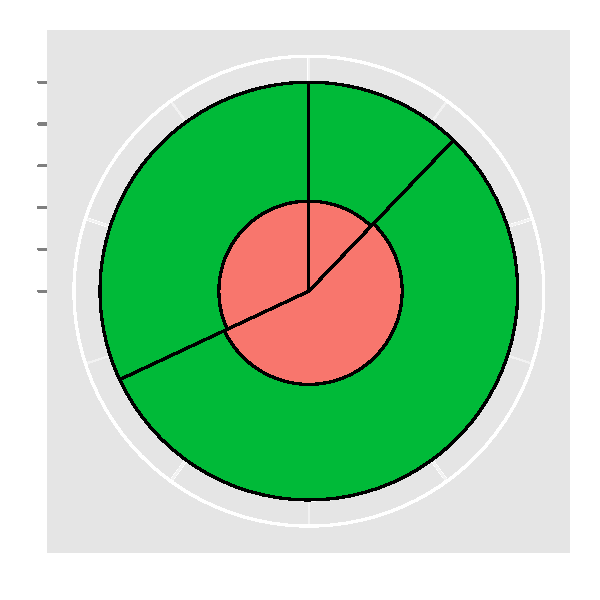
\includegraphics[width=0.25\linewidth]{hs-vs-polar}

    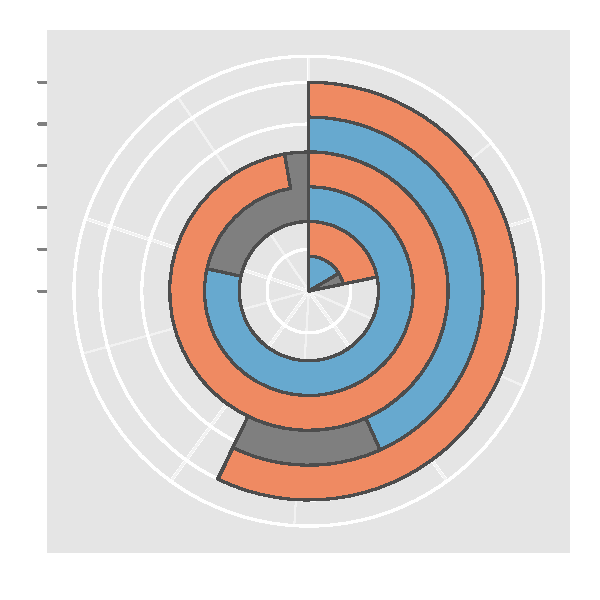
\includegraphics[width=0.25\linewidth]{hb-vb-polar-2}%
    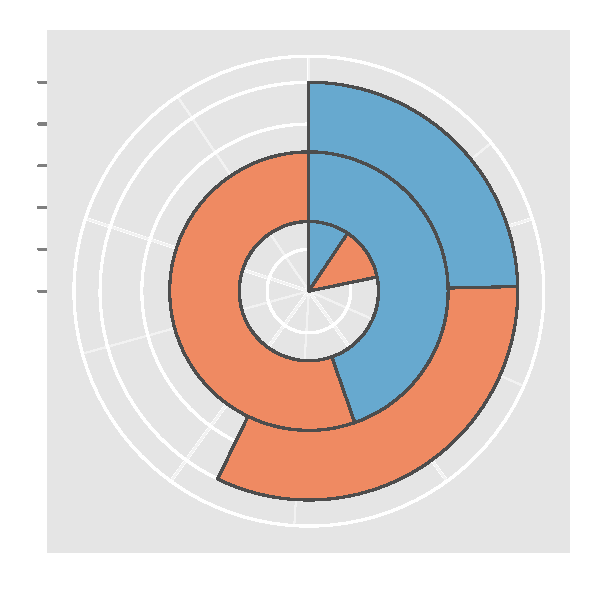
\includegraphics[width=0.25\linewidth]{hb-vs-polar-2}%
    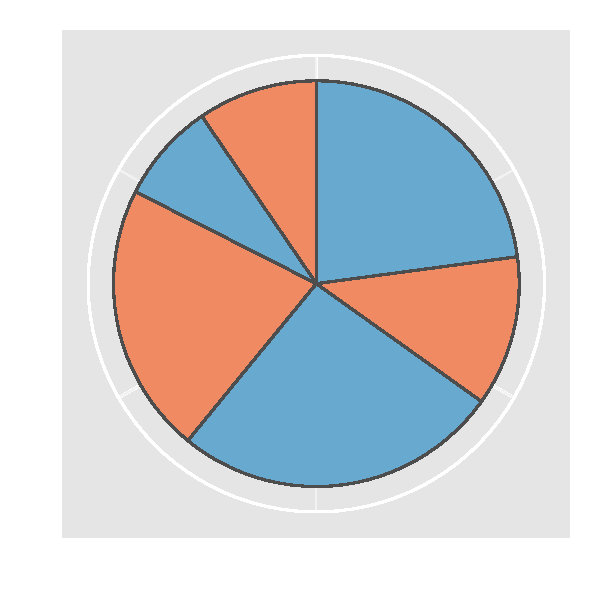
\includegraphics[width=0.25\linewidth]{hs-hs-polar-2}%
    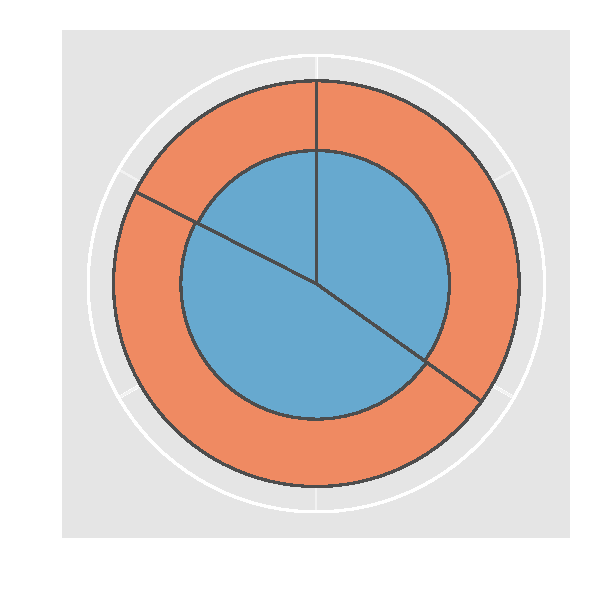
\includegraphics[width=0.25\linewidth]{hs-vs-polar-2}

  \caption{(Top) Area graphics in Cartesian coordinates. (Mid) Area graphics in polar coordinates. (Bottom) Product graphics with alternate mapping of $x$ and $y$ to $r$ and $\theta$. From left to right: hbar + hbar, vspline + hbar, hspine + hspine, hspine + vspine. (\key{male} male, \key{female} female)}

  \label{fig:polar}
\end{figure}

Other non-rectangular area graphics include non-rectangular treemaps, such as circular treemaps \citep{wetzel:2008}, space-filling curves \citep{wattenberg:2005} and voronoi treemaps \citep{balzer:2005}.

\section{R package}
\label{sec:package}

We have provided a reference implementation of these ideas in an R \citep{R} package called {\tt productplots}, available from {\tt http://github.com/hadley/productplots}. There are two main functions: {\tt prodcalc}, which computes the coordinates of each rectangle; and {\tt prodplot}, which displays the rectangles with the ggplot2 package \citep{me:ggplot2}. The code is well tested, and ensures that the constraints are always satisfied. 

For example, the following code conveys the essence of the plots in Figure~\ref{fig:part-cond}. The function {\tt prodplot} creates plots of the {\tt happy} data, defined using the standard R formula notation (\verb|~|), with the convention that {\tt |} denotes conditioning. The final argument lists the graphical primitives to use for display. This can also be a template function like {\tt mosaic()} which produces a standard, named, graphic.

\begin{verbatim}
prodplot(happy, ~ happy + finrela + health, 
  c("vspine", "fluct"))
prodplot(happy, ~ happy | finrela + health, 
  c("vspine", "fluct"))
prodplot(happy, ~ happy | finrela + health, 
  c("hspine", "fluct"))
\end{verbatim}

As for all presentation graphics, the actual code is somewhat more complicated, as we make a number of tweaks for optimal display. The complete {\tt productplots} code to used to create the images in this paper is available from the authors upon request. 

The {\tt productplots} package has been designed to be flexible and extensive.  For example, each graphical primitive is represented by a function: {\tt hspine()}, {\tt vspine()}, {\tt spine()}, {\tt hbar()}, {\tt vbar()}, {\tt tile()} and {\tt fluct()}. Adding a new graphical primitive is easy: you just write a new function, and can use the existing calculation and display algorithms.

\section{Conclusion}
\label{sec:conclusion}

The product plots framework is successful at describing many existing graphics that display tables of counts, proportions and probabilities. It lays the framework for much future work, particularly because the framework leads to a combinatorial explosion of possibilities. For example, a 4d {\sc pmf}, $f(a, b, c, d)$, can be factorised in five different ways:

\begin{itemize}
  \setlength{\itemsep}{0em}
  
  \item $f(a, b, c, d) = f(a | b, c, d) f(b | c, d) f(c | d) f(d)$
  \item $f(a, b, c, d) = f(a | b, c, d) f(b | c, d) f(c, d)$
  \item $f(a, b, c, d) = f(a | b, c, d) f(b, c | d) f(d)$
  \item $f(a, b, c, d) = f(a, b | c, d) f(c | d) f(d)$
  \item $f(a, b, c, d) = f(a, b | c, d) f(c, d)$
\end{itemize}

\noindent There are 24 possible ways of ordering the variables in the {\sc pmf}, 5 ways of displaying a 1d {\sc pmf}, and 1 way of displaying a 2d {\sc pmf}, leading to a possible $24 * (5^4 + 5^2 + 5^2 + 5^2 + 1) = 16,824$ plots, before we even consider conditioning! The product plots framework defines a large space of potential plots.

Well thought out interaction will make it easier to navigate this space, and we have begun to develop a prototype model in R, as part of the cranvas suite of interactive graphics, {\tt http://github.com/ggobi/cranvas}.  However, much work and user testing remains to be done before we can be confident that we have developed a useful navigation model.

We are also exploring the connection between product plots and log-linear (aka Poisson) models, the statistical models most commonly used for count data. Some special cases of the general connection have already been worked out. For example, \citep{hofmann:2003} shows how looking for straight lines in a mosaic plot corresponds to a formal test of independence between two variables. Generally, we are interested in knowing what visual comparisons are equivalent to what formal statistical tests, and conversely, how significant coefficients in a model can help us choose a set of useful plots. Given a question, can we suggest appropriate plots? Given a plot, can we suggest questions that it might answer?

Product plots also need to be extended with systematic ways of displaying uncertainty, to help users identify whether differences in the plot represent real differences in the underlying population or are just the result of random variation. This is particularly important because area plots typically have fixed area, meaning that the total number of observations in a plot is not directly displayed, even though this is crucial for determining whether a difference is statistically significant or not.

Finally, continuous data is currently incorporated in a simplistic manner. Can we extend the product plots framework to include plots designed to show continuous distributions like the average shifted histogram \citep{scott:1985} or the kernel density estimate \citep{scott:1992}?

\acknowledgments{Computations performed in R \citep{R} and graphics produced with ggplot2 \citep{me:ggplot2}.}

% bibtool -x prodplots-infovis > references.bib
\bibliographystyle{ieeetr}
\bibliography{references}

\end{document}
